\chapter{Background}

This chapter concludes the fundamental knowledge that is needed to comprehend the upcoming practical work. Firstly, an introduction to cloud computing will be held. Next, a throrough understanding of honeypots is given. Lastly, we introduce some concepts of intrusion detection systens.

\section{Cloud Computing}

Nowadays it is one of the well-known keywords and has been used by vary large companies such as Google, or Amazon, however, the term \enquote{cloud computing} dates back to the late 1996, when a small group of technology executives of Compaq Computer framed new business ideas around the Internet.\cite{regalado2020} Starting from 2007 cloud computing evolved into a serious competitor and outnumbered the keywords \enquote{virtualization}, and \enquote{grid computing} reported by Google trends \cite{Wang2010}. Shortly, various cloud provider become publicly available, each with their own strengths and weaknesses. For example IBM's Cloud\footnote{\url{https://www.ibm.com/cloud}}, Amazon Web Services\footnote{\url{https://aws.amazon.com/}}, and Google Cloud\footnote{\url{https://cloud.google.com/}}. Why are clouds so attractive in practice?

\begin{itemize}
    \item s
    \item s
    \item s
\end{itemize}

In this section, we want to give basic unterstandings of cloud computing, and give an short introduction to HeiCloud.

\subsection{Definition of Cloud Computing}

Considering the definition of Brian Hayes, cloud computing is \enquote{a shift in the geography of computation} \cite{hayes2008}. Thus, computational workload is moved away from local instances towards services and datacenters that provide the need of users \cite{Armbrust2010}.

Considering the definition of the \ac{nist}, cloud computing \enquote{is a model for enabling ubiquitous, convenient, on-demand network access to a shared pool of configurable computing resources (e.g., networks, servers, storage, applications, and services) that can be rapidly provisioned and released with minimal management effort or service provider interaction} \cite{Mell2011}. \ac{nist} not only reflects the geographical shift of resources such as datacenters, but also mentions on-demand usage that contributes to a flexible resource management. Morever, \ac{nist} composes the term in five essential characteristics, three service models (see \ref{subsec:cloud-service}), and four deployment models (see \ref{subsec:cloud-deployment}):\\

\textit{On-demand-self-service} refers to the unilaterally provision computing capabilities. Consumers can acquire server time and network storage on demand without a human interaction.\\

\textit{Broad network access} characterizes the access of capabilities of the network through standard protocols such as \ac{http}. Heterogeneous thin and thick client platforms should be supported.\\

\textit{Resource pooling} allows the provider's computing resources to be pooled across several consumers. A multi-tanent model with different physical and virtual resources are assigned on demand. Other aspects such as location are independent and cannot be controlled on a low-level by consumers. Moreover, high-level access to specify continent, state, or datacenter can be available.\\

\textit{Rapid elasticity} offers consumers to extend and release capabilities easily. Further automization to quickly increase resources  when demand skyrockets significantly can be supported regardless limit and quantity at any time.\\

\textit{Measured service} handles resources in an automated and optimized manner. It uses additional metering capabilities to trace storage, processing, bandwith, and active user accounts. This helps to monitor, and control resource usage. Thus, contributing to transparency between provider and consumer.

\subsection{Service models}
\label{subsec:cloud-service}

\ac{saas} \\

\ac{paas}\\

\ac{iaas}\\

\ac{daas}\\

\begin{figure}[h]
    \centering
    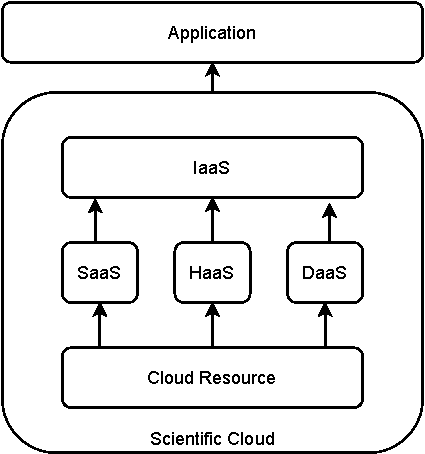
\includegraphics[width=0.4\textwidth]{figures/cloud-functionalities.pdf}
    \caption{Cloud functionalities (derived from \cite{Wang2010})}
    \label{fig:mesh1}
\end{figure}


Examples for such service models are:

\subsection{Deployment models}
\label{subsec:cloud-deployment}

Private Cloud\\

Community Cloud\\

Public Cloud\\

Hybrid Cloud\\

Examples for such deployment models are:

\subsection{Cloud Security}

\cite{Nithin2012}

\subsection{HeiCloud}

\section{Honeypots}

The first public honeypot \cite{Spitzner2003}

\subsection{Definition of a Honeypot}

On the Internet there are a dozen of defintions for honeypots. Thus, to cope with all the subtle differences, we want to take a closer look at some of the definitions and narrow down our own one.

Spitzner defines honeypots as a \enquote{security resource whose value lies in being probed, attacked, or compromised.}\cite{Spitzner2003}

High-interaction honeypots\\

Low-interaction honeypots\\

Pure honeypots\\

%\subsection{Honeyd}

%\subsection{Configuration Honeyd}

\subsection{Honeynets}

\cite{Spitzner2003}

\subsection{Legal Issues}

\cite{Spitzner2003}

\section{Intrusion Detection System}
